% Provenance (never printed): old premiere S / seconde material on minerals and
% rocks (identifying minerals in hand specimen, the silicates, the minerals of
% granite, basalt and peridotite, thin sections in polarised light).
% Element fractions and rock densities from figdata/grade-11/mineral_density.py
% (Rudnick and Gao 2014 bulk crust; webmineral mean densities). Mineral, crystal,
% rock families and the Mohs scale are Book 1's (grade 6): recalled, not defined.
% Felsic and mafic belong to g11.08: not used here.
\chapter{Les minéraux}\label{ch:g11:minerals}

Ramassez un galet de granite et regardez-le à la loupe. Ce n'est pas une
seule substance, mais une mosaïque de grains imbriqués~: des grains gris,
vitreux et presque transparents~; des grains roses, trapus, dont les faces
cassées lancent des éclairs quand on tourne le galet~; de petites paillettes
noires que la pointe d'un couteau détache en feuillets minces. Chaque sorte
de grain est un minéral. Ce chapitre montre comment un géologue les
distingue, pourquoi presque tous sont bâtis à partir de silicium et
d'oxygène, comment ils forment les roches rencontrées jusqu'ici --- granite,
basalte, \omterm{def:g11:ocean-ridges:peridotite}{péridotite} --- et comment une tranche de roche plus fine qu'un
cheveu, vue en lumière polarisée, les montre tous à la fois.

\begin{omfigure}
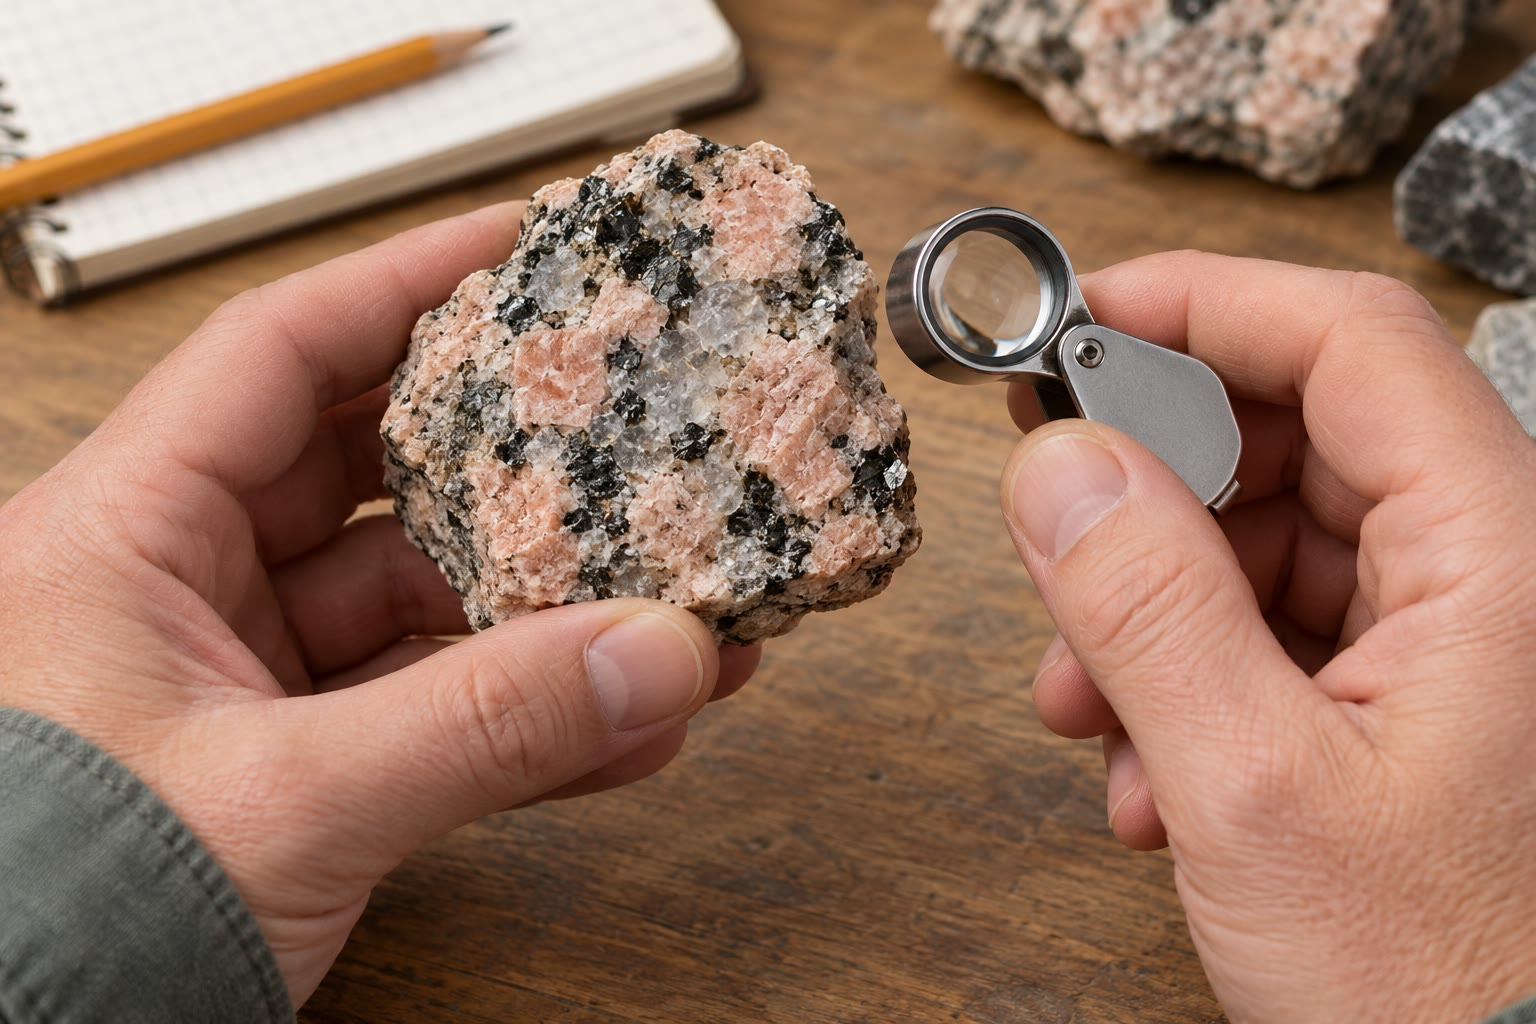
\includegraphics[width=0.62\linewidth]{images/book2/ai/g11-geologist-hand-lens.jpg}

{\small Un granite examiné à la loupe~: le premier outil pour distinguer les
minéraux. (Illustration générée par IA.)}
\end{omfigure}

\begin{recall}
Un minéral est une substance solide naturelle, non produite par les êtres
vivants, de composition définie et dont les atomes sont disposés de façon
régulière~; une roche est faite d'un ou de plusieurs minéraux. Le granite
est fait surtout de feldspath, de quartz et de mica. Les roches se rangent
en trois familles, magmatiques (ou ignées), sédimentaires et métamorphiques.
La dureté d'un minéral est sa résistance à la rayure, classée de 1 (talc) à
10 (diamant) sur l'échelle de Mohs~; le feldspath orthose vaut 6 et le
quartz 7, alors qu'une plaque de verre vaut environ 5.5 et un clou d'acier
environ 6.5 (livre~1, année~6). La masse volumique d'un corps est sa masse
divisée par son volume (les livres de physique). Un composé est décrit par
une formule qui compte ses atomes~; dans un solide fait d'ions, les charges
positives et négatives se compensent (les livres de chimie). La \omterm{def:g11:ocean-ridges:peridotite}{péridotite}
forme le manteau~; le \omterm{def:g11:ocean-ridges:gabbro}{gabbro} et le basalte forment la \omterm{def:g11:ocean-ridges:oceanic-lithosphere}{croûte océanique}
(\cref{ch:g11:ocean-ridges}).
\end{recall}
% ledger: usgs:mineral-rock, nps:granite-minerals, nps:mohs-ladder, nps:mohs-testers

\section{Distinguer les minéraux}

Un minéral a une composition définie et un arrangement régulier d'atomes.
Les deux se voient de l'extérieur~: dans la forme de ses cristaux, sa façon
de se casser, sa façon de réfléchir la lumière, sa dureté et sa masse
volumique. Aucune de ces propriétés ne suffit seule~; ensemble, elles
permettent d'identifier les minéraux courants sur un échantillon à la main,
sans autre instrument qu'une loupe, un clou d'acier et une plaque de verre.

\paragraph{La forme.} Un cristal qui a grandi librement, dans une cavité ou
dans un liquide, prend une forme qui reflète l'arrangement de ses atomes.

\begin{definition}[Habitus]\label{def:g11:minerals:habit}
L'\emph{habitus}\index{habitus (d'un cristal)} d'un minéral est la forme
générale que prennent ses cristaux~: cubique, tabulaire (plat, comme une
tablette), prismatique (allongé, comme un prisme), en lames, aciculaire (en
aiguilles), etc.
\end{definition}
% ledger: tulane:physprop

Le quartz croît en prismes à six faces terminés en pointe~; la biotite, en
plaques plates à six côtés (photographies ci-dessous). Dans la plupart des
roches, pourtant, les grains ont grandi les uns contre les autres et n'ont
pas de faces propres~: l'\omterm{def:g11:minerals:habit}{habitus} renseigne alors peu, et les autres
propriétés prennent le relais.
% ledger: photo:g11-quartz, photo:g11-biotite

\paragraph{La couleur et l'éclat.} La couleur est la première chose que l'on
voit, et la moins fiable. Une trace d'un autre élément suffit à la changer~:
le quartz peut être incolore, blanc, noir, rose, bleu ou violet. Quelques
minéraux, en revanche, varient peu~: l'olivine est presque toujours verte.
La façon dont un minéral réfléchit la lumière est un meilleur guide.
% ledger: tulane:physprop

\begin{definition}[Éclat]\label{def:g11:minerals:lustre}
L'\emph{éclat}\index{eclat@éclat} d'un minéral est son aspect en lumière
réfléchie. Il est \emph{métallique} quand le minéral brille comme un métal,
et non métallique sinon~: \emph{vitreux} (comme du verre, tel le quartz),
nacré, résineux, etc.
\end{definition}
% ledger: tulane:physprop

\paragraph{La façon de se casser.} Frappez un cristal~: il se casse. Là où
les liaisons entre ses atomes sont plus faibles selon certains plans, il se
fend selon ces plans, encore et encore, en surfaces planes et brillantes~;
là où aucun plan n'est plus faible qu'un autre, il se casse selon une
surface quelconque.

\begin{definition}[Clivage~; cassure]\label{def:g11:minerals:cleavage}
Le \emph{clivage}\index{clivage (d'un mineral)@clivage (d'un minéral)} est
la tendance d'un minéral à se casser selon des plans, parallèles à des
directions dans lesquelles les liaisons entre ses atomes sont plus faibles.
La \emph{cassure}\index{cassure (d'un mineral)@cassure (d'un minéral)} est
une rupture selon des surfaces irrégulières, dans un minéral sans plan de
faiblesse~; une cassure à surfaces lisses et courbes, comme celle du verre
brisé, est dite \emph{conchoïdale}.
\end{definition}
% ledger: tulane:physprop

Un minéral peut avoir un \omterm{def:g11:minerals:cleavage}{clivage}, deux, trois ou aucun. Les micas en ont un,
parfait~: ils se détachent en feuillets. Les feldspaths en ont deux. Le
quartz n'en a aucun~: il se casse avec une \omterm{def:g11:minerals:cleavage}{cassure} conchoïdale, ce qui le
distingue aussitôt d'un feldspath de même couleur grise ou blanche. L'angle
entre deux \omterm{def:g11:minerals:cleavage}{clivages} est fixé par l'arrangement des atomes, et on peut le
mesurer sur un grain cassé ou sur une section~: les deux \omterm{def:g11:minerals:cleavage}{clivages} d'un
pyroxène se coupent à environ \ang{87} et \ang{93}, presque à angle droit~;
ceux d'une amphibole à environ \ang{56} et \ang{124}. Les pyroxènes et les
amphiboles sont souvent sombres et semblables~; leurs angles de \omterm{def:g11:minerals:cleavage}{clivage} les
distinguent.
% ledger: wm:densities (quartz conchoidal; orthoclase two cleavages; biotite one), tulane:cleavage-angles

\begin{omfigure}
\begin{tikzpicture}[font=\footnotesize]
  % pyroxene: octagonal cross-section, cleavage traces at 46.5 and 133.5 degrees (87/93)
  \begin{scope}
    \coordinate (p1) at (1,0.4); \coordinate (p2) at (0.431,1); \coordinate (p3) at (-0.431,1);
    \coordinate (p4) at (-1,0.4); \coordinate (p5) at (-1,-0.4); \coordinate (p6) at (-0.431,-1);
    \coordinate (p7) at (0.431,-1); \coordinate (p8) at (1,-0.4);
    \begin{scope}[scale=1.5]
      \fill[black!72!green!40] (1,0.4) -- (0.431,1) -- (-0.431,1) -- (-1,0.4) -- (-1,-0.4) -- (-0.431,-1) -- (0.431,-1) -- (1,-0.4) -- cycle;
      \clip (1,0.4) -- (0.431,1) -- (-0.431,1) -- (-1,0.4) -- (-1,-0.4) -- (-0.431,-1) -- (0.431,-1) -- (1,-0.4) -- cycle;
      \foreach \s in {-5,...,5} {
        \draw[white!85!black, line width=0.5pt] ($(136.5:\s*0.24)+(46.5:-3)$) -- ($(136.5:\s*0.24)+(46.5:3)$);
        \draw[white!85!black, line width=0.5pt] ($(223.5:\s*0.24)+(133.5:-3)$) -- ($(223.5:\s*0.24)+(133.5:3)$);}
      \draw[black!80, line width=0.9pt] (46.5:-3) -- (46.5:3); \draw[black!80, line width=0.9pt] (133.5:-3) -- (133.5:3);
    \end{scope}
    \draw[black!70, line width=0.7pt, scale=1.5] (1,0.4) -- (0.431,1) -- (-0.431,1) -- (-1,0.4) -- (-1,-0.4) -- (-0.431,-1) -- (0.431,-1) -- (1,-0.4) -- cycle;
    \draw[omProp, line width=1pt] (46.5:0.75) arc[start angle=46.5, end angle=133.5, radius=0.75];
    \draw[omDef, line width=1pt] (133.5:0.5) arc[start angle=133.5, end angle=226.5, radius=0.5];
    \node[fill=white, inner sep=1pt, text=omProp!80!black] at (90:0.98) {\ang{87}};
    \node[fill=white, inner sep=1pt, text=omDef] at (180:0.82) {\ang{93}};
    \node[anchor=north, align=center] at (0,-1.7) {\strut\textbf{pyroxène}\\clivages à environ \ang{87} et \ang{93}};
  \end{scope}
  % amphibole: elongated hexagon, cleavage traces at 28 and 152 degrees (56/124 opening sideways)
  \begin{scope}[xshift=6.2cm]
    \begin{scope}[scale=1.5]
      \fill[black!72!green!40] (1.6,0) -- (0.62,0.52) -- (-0.62,0.52) -- (-1.6,0) -- (-0.62,-0.52) -- (0.62,-0.52) -- cycle;
      \clip (1.6,0) -- (0.62,0.52) -- (-0.62,0.52) -- (-1.6,0) -- (-0.62,-0.52) -- (0.62,-0.52) -- cycle;
      \foreach \s in {-6,...,6} {
        \draw[white!85!black, line width=0.5pt] ($(118:\s*0.2)+(28:-4)$) -- ($(118:\s*0.2)+(28:4)$);
        \draw[white!85!black, line width=0.5pt] ($(242:\s*0.2)+(152:-4)$) -- ($(242:\s*0.2)+(152:4)$);}
      \draw[black!80, line width=0.9pt] (28:-4) -- (28:4); \draw[black!80, line width=0.9pt] (152:-4) -- (152:4);
    \end{scope}
    \draw[black!70, line width=0.7pt, scale=1.5] (1.6,0) -- (0.62,0.52) -- (-0.62,0.52) -- (-1.6,0) -- (-0.62,-0.52) -- (0.62,-0.52) -- cycle;
    \draw[omProp, line width=1pt] (-28:0.75) arc[start angle=-28, end angle=28, radius=0.75];
    \draw[omDef, line width=1pt] (28:0.42) arc[start angle=28, end angle=152, radius=0.42];
    \node[fill=white, inner sep=1pt, text=omProp!80!black] at (0:1.02) {\ang{56}};
    \node[fill=white, inner sep=1pt, text=omDef] at (90:0.6) {\ang{124}};
    \node[anchor=north, align=center] at (0,-1.7) {\strut\textbf{amphibole}\\clivages à environ \ang{56} et \ang{124}};
  \end{scope}
\end{tikzpicture}

{\small Sections d'un cristal de pyroxène (à gauche) et d'un cristal
d'amphibole (à droite), coupés perpendiculairement à leur longueur
(schéma). Les traits fins sont les traces des deux \omterm{def:g11:minerals:cleavage}{clivages}, dont deux sont
tracés plus épais là où on lit les angles~; les angles qu'ils forment,
presque droits dans le pyroxène, bien plus ouverts et bien plus fermés dans
l'amphibole, distinguent deux minéraux sombres par ailleurs semblables.}
\end{omfigure}
% ledger: tulane:cleavage-angles

\paragraph{La dureté et la masse volumique.} La dureté, vue dans le
livre~1, sépare des minéraux qui se ressemblent~: le quartz (7) raye le
verre et n'est pas rayé par un clou d'acier~; un feldspath (6) raye aussi le
verre, mais le clou le raye. La masse volumique est le dernier indice. On
ne peut pas peser un grain à la main, mais on peut peser un échantillon fait
d'un seul minéral, et les minéraux courants des roches couvrent un
intervalle étroit, d'environ \qty{2.6}{g/cm^3} à environ \qty{3.4}{g/cm^3}
(graphique ci-dessous)~: les plus légers sont riches en silicium, en
aluminium, en sodium et en potassium, les plus denses en fer et en
magnésium.
% ledger: nps:mohs-ladder, nps:mohs-testers, wm:densities

\begin{method}[Identifier un minéral sur un échantillon à la main]\label{met:g11:minerals:identify}
\begin{enumerate}
  \item Observer la forme du grain ou du cristal (\omterm{def:g11:minerals:habit}{habitus}), sa couleur ---
        à titre d'indice seulement --- et son \omterm{def:g11:minerals:lustre}{éclat}.
  \item Chercher un \omterm{def:g11:minerals:cleavage}{clivage}~: des surfaces planes et brillantes qui
        accrochent la lumière ensemble quand on tourne l'échantillon.
        Compter les directions de \omterm{def:g11:minerals:cleavage}{clivage} et estimer l'angle qu'elles
        forment~; s'il n'y en a aucune, décrire la \omterm{def:g11:minerals:cleavage}{cassure}.
  \item Tester la dureté à l'aide d'objets de référence~: une plaque de
        verre (environ 5.5) et un clou d'acier (environ 6.5).
  \item Si l'échantillon est fait d'un seul minéral, comparer sa masse
        volumique à celles des candidats.
  \item Conclure par la combinaison des propriétés, jamais par une seule.
\end{enumerate}
\end{method}
% ledger: nps:mohs-testers

\begin{example}[Quartz ou feldspath~?]
Deux grains gris-blanc dans un granite. Le premier ne montre aucune face
plane, seulement des \omterm{def:g11:minerals:cleavage}{cassures} lisses et courbes, et le clou d'acier n'y
laisse aucune trace~: \omterm{def:g11:minerals:cleavage}{cassure} conchoïdale et dureté supérieure à 6.5, c'est
du quartz (7). Le second se casse en surfaces planes et brillantes selon
deux directions et il est rayé par le clou, bien qu'il raye le verre~: deux
\omterm{def:g11:minerals:cleavage}{clivages} et une dureté comprise entre 5.5 et 6.5, c'est un feldspath (6).
\end{example}
% ledger: wm:densities, nps:mohs-ladder, nps:mohs-testers

\begin{omfigure}
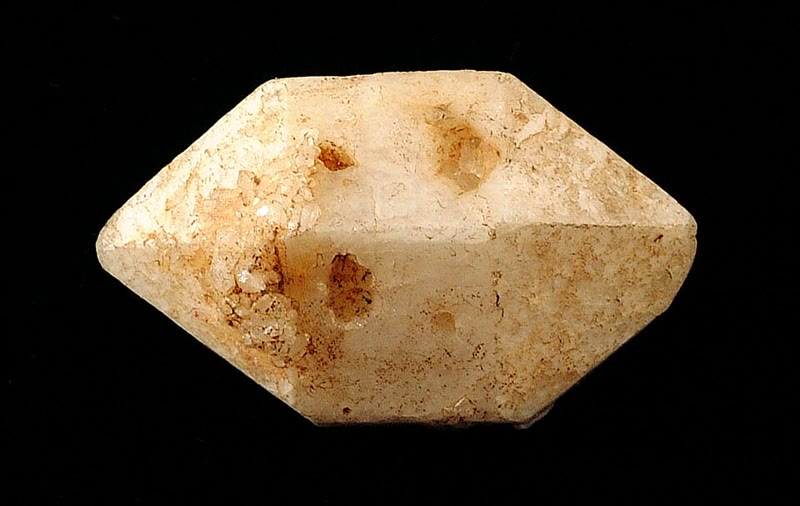
\includegraphics[height=2.75cm]{images/book2/g11-geodil-quartz.jpg}\hfill
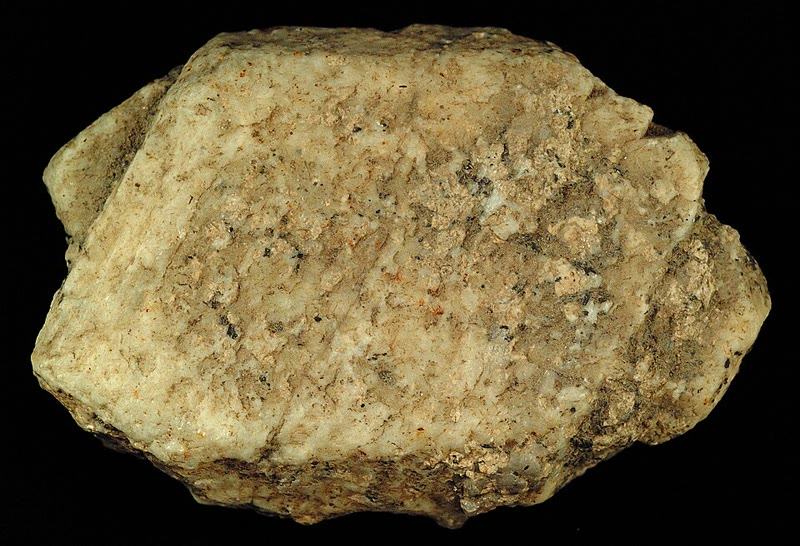
\includegraphics[height=2.75cm]{images/book2/g11-geodil-orthoclase.jpg}\hfill
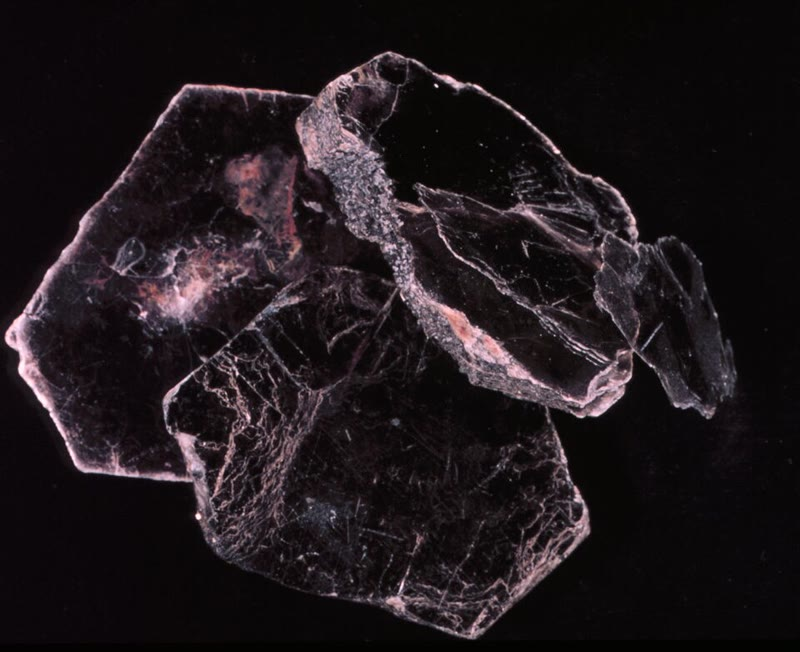
\includegraphics[height=2.75cm]{images/book2/g11-geodil-biotite.jpg}\hfill
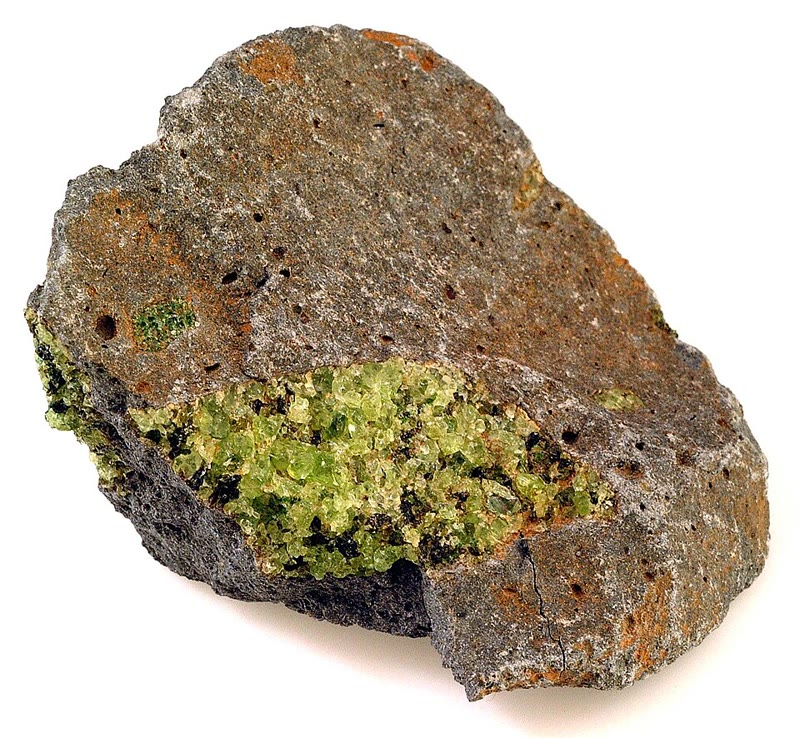
\includegraphics[height=2.75cm]{images/book2/g11-geodil-olivine.jpg}

{\small Quatre minéraux des roches. De gauche à droite~: un cristal de
quartz, un prisme à six faces terminé en pointe aux deux bouts, long
d'environ \qty{5}{cm}~; un feldspath orthose, deux cristaux soudés, environ
\qty{7}{cm}~; des plaques à six côtés de mica biotite, environ \qty{6}{cm},
qui se détachent en feuillets minces selon leur unique \omterm{def:g11:minerals:cleavage}{clivage}~; des grains
verts d'olivine dans un basalte. Photographies Shannon Heinle, Darla
Sondrol, Dexter Perkins et Nessa Eull, Geology Digital Image Library (CC0).}
\end{omfigure}
% ledger: photo:g11-quartz, photo:g11-orthoclase, photo:g11-biotite, photo:g11-olivine

\section{Les silicates}

\paragraph{Deux éléments forment la croûte.} La composition chimique de la
croûte continentale est connue grâce aux analyses de nombreuses roches,
exprimées en pourcentages d'oxydes~: environ \qty{60.6}{\percent} de
\ce{SiO2}, \qty{15.9}{\percent} d'\ce{Al2O3}, etc. On en déduit, avec les
masses des atomes, la masse de chaque élément. L'oxygène représente
\qty{46}{\percent} de la masse de la croûte continentale et le silicium
\qty{28}{\percent}~: deux éléments, environ les trois quarts de la masse.
Avec six métaux --- aluminium, fer, calcium, magnésium, sodium et
potassium ---, ils en forment plus de \qty{99}{\percent}.
% ledger: rg14:crust, ciaaw:O, ciaaw:Si, ciaaw:Al, ciaaw:Fe, ciaaw:Ca, ciaaw:Mg, ciaaw:Na, ciaaw:K, ciaaw:Ti, ciaaw:Mn, ciaaw:P
% values (mineral_density.py): bulk_O 46.36, bulk_Si 28.30, O+Si 74.66, eight elements 99.43

\begin{omfigure}
\begin{tikzpicture}
\begin{axis}[omrecord, width=0.82\linewidth, height=5.6cm, ybar, bar width=14pt,
  ymin=0, ymax=55, xtick=data, enlarge x limits=0.06,
  xticklabels from table={figdata/out/grade-11-mineral_density-elements.dat}{symbol},
  ylabel={part de la masse (\unit{\percent})},
  nodes near coords, every node near coord/.append style={font=\scriptsize, /pgf/number format/.cd, fixed, precision=1},
  xmajorgrids=false]
% computed in figdata/grade-11/mineral_density.py; ledger: rg14:crust, ciaaw:*
\addplot[fill=omDef!55, draw=omDef] table[x expr=\coordindex, y=frac] {figdata/out/grade-11-mineral_density-elements.dat};
\end{axis}
\end{tikzpicture}

{\small Les éléments de la croûte continentale, en parts de sa masse,
calculées à partir de sa composition moyenne en oxydes (Rudnick et Gao,
2014). L'oxygène et le silicium forment à eux seuls environ les trois quarts
de la masse.}
\end{omfigure}

\paragraph{Le tétraèdre silicium--oxygène.} Un atome de silicium est petit,
et quatre atomes d'oxygène tiennent autour de lui, aux sommets d'un
tétraèdre, une pyramide à quatre faces triangulaires. Le groupe contient un
ion silicium \ce{Si^4+} et quatre ions oxygène \ce{O^2-}~: il porte une
charge de $4 - 4 \times 2 = -4$, que d'autres ions --- ou d'autres
tétraèdres --- doivent compenser.

\begin{definition}[Silicate~; tétraèdre silicium--oxygène]\label{def:g11:minerals:silicate}
Le \emph{tétraèdre silicium--oxygène}\index{tetraedre silicium--oxygene@tétraèdre silicium--oxygène}
est le groupe \ce{SiO4} formé par un atome de silicium et les quatre atomes
d'oxygène qui l'entourent, aux sommets d'un tétraèdre. Un
\emph{silicate}\index{silicate} est un minéral bâti à partir de tétraèdres
silicium--oxygène, isolés ou reliés les uns aux autres par des sommets
communs.
\end{definition}
% ledger: tulane:silicates

Les tétraèdres se relient en partageant des oxygènes~: le sommet d'un
tétraèdre est le sommet du suivant. Le nombre de sommets que partage chaque
tétraèdre fixe la structure du \omterm{def:g11:minerals:silicate}{silicate}, et sa formule.
\begin{itemize}
  \item \emph{Tétraèdres isolés}, ne partageant aucun sommet, maintenus
        ensemble par des ions métalliques situés entre eux~: l'olivine,
        \ce{(Mg,Fe)2SiO4}.
  \item \emph{Chaînes simples}, chaque tétraèdre partageant deux sommets
        avec ses voisins~: les pyroxènes.
  \item \emph{Chaînes doubles}, deux chaînes simples accolées, les
        tétraèdres partageant tour à tour deux ou trois sommets~: les
        amphiboles.
  \item \emph{Feuillets}, chaque tétraèdre partageant trois sommets~: les
        micas, et les \omterm{def:g10:soil-formation:clay}{minéraux argileux} des sols
        (\cref{ch:g10:soil-formation}).
  \item \emph{Charpentes}, chaque tétraèdre partageant ses quatre sommets,
        dans les trois directions de l'espace~: le quartz, \ce{SiO2}, et ---
        avec de l'aluminium à la place d'une partie du silicium --- les
        feldspaths.
\end{itemize}
% ledger: tulane:silicates

\begin{omfigure}
\begin{tikzpicture}[font=\footnotesize]
  % coordinates generated once by a small script (scratch, not kept): kagome net of side 0.62 cm,
  % a regular tetrahedron in perspective, and a framework piece of five tetrahedra (painter's order)
  % (a) one SiO4 tetrahedron, drawn in perspective; the silicon (black) at its centre
  \fill[omDef!12] (2.300,2.979) -- (1.927,1.372) -- (1.221,0.629) -- (3.752,0.820) -- cycle;
  \draw[densely dashed, omDef!60, line width=0.6pt] (2.300,2.979) -- (1.927,1.372);
  \draw[omDef!70!black, line width=0.6pt] (2.300,2.979) -- (1.221,0.629);
  \draw[omDef!70!black, line width=0.6pt] (2.300,2.979) -- (3.752,0.820);
  \draw[densely dashed, omDef!60, line width=0.6pt] (1.927,1.372) -- (1.221,0.629);
  \draw[densely dashed, omDef!60, line width=0.6pt] (1.927,1.372) -- (3.752,0.820);
  \draw[omDef!70!black, line width=0.6pt] (1.221,0.629) -- (3.752,0.820);
  \draw[black!55, line width=0.4pt] (2.300,1.450) -- (2.300,2.979);
  \draw[black!55, line width=0.4pt] (2.300,1.450) -- (1.927,1.372);
  \draw[black!55, line width=0.4pt] (2.300,1.450) -- (1.221,0.629);
  \draw[black!55, line width=0.4pt] (2.300,1.450) -- (3.752,0.820);
  \fill[black] (2.300,1.450) circle (2.2pt);
  \filldraw[fill=omThm!35, draw=omThm!80!black, line width=0.4pt] (2.300,2.979) circle (4.2pt);
  \filldraw[fill=omThm!35, draw=omThm!80!black, line width=0.4pt] (1.927,1.372) circle (4.2pt);
  \filldraw[fill=omThm!35, draw=omThm!80!black, line width=0.4pt] (1.221,0.629) circle (4.2pt);
  \filldraw[fill=omThm!35, draw=omThm!80!black, line width=0.4pt] (3.752,0.820) circle (4.2pt);
  % coordinates for labels: Si 2.300,1.450; apex 2.300,2.979
  % (b) isolated tetrahedra (olivine)
  \filldraw[fill=omDef!22, draw=omDef!70!black, line width=0.5pt] (6.200,0.900) -- (6.820,0.900) -- (6.510,1.437) -- cycle;
  \fill[black] (6.510,1.079) circle (0.9pt);
  \filldraw[fill=omDef!22, draw=omDef!70!black, line width=0.5pt] (8.370,1.437) -- (8.990,1.437) -- (8.680,1.974) -- cycle;
  \fill[black] (8.680,1.616) circle (0.9pt);
  \filldraw[fill=omDef!22, draw=omDef!70!black, line width=0.5pt] (8.060,1.974) -- (7.750,2.511) -- (8.370,2.511) -- cycle;
  \fill[black] (8.060,2.332) circle (0.9pt);
  \filldraw[fill=omDef!22, draw=omDef!70!black, line width=0.5pt] (8.990,0.363) -- (9.610,0.363) -- (9.300,0.900) -- cycle;
  \fill[black] (9.300,0.542) circle (0.9pt);
  \filldraw[fill=omDef!22, draw=omDef!70!black, line width=0.5pt] (9.920,1.974) -- (9.610,2.511) -- (10.230,2.511) -- cycle;
  \fill[black] (9.920,2.332) circle (0.9pt);
  \filldraw[fill=omThm!35, draw=omThm!80!black, line width=0.4pt] (6.200,0.900) circle (1.9pt);
  \filldraw[fill=omThm!35, draw=omThm!80!black, line width=0.4pt] (6.510,1.437) circle (1.9pt);
  \filldraw[fill=omThm!35, draw=omThm!80!black, line width=0.4pt] (6.820,0.900) circle (1.9pt);
  \filldraw[fill=omThm!35, draw=omThm!80!black, line width=0.4pt] (7.750,2.511) circle (1.9pt);
  \filldraw[fill=omThm!35, draw=omThm!80!black, line width=0.4pt] (8.060,1.974) circle (1.9pt);
  \filldraw[fill=omThm!35, draw=omThm!80!black, line width=0.4pt] (8.370,2.511) circle (1.9pt);
  \filldraw[fill=omThm!35, draw=omThm!80!black, line width=0.4pt] (8.370,1.437) circle (1.9pt);
  \filldraw[fill=omThm!35, draw=omThm!80!black, line width=0.4pt] (8.680,1.974) circle (1.9pt);
  \filldraw[fill=omThm!35, draw=omThm!80!black, line width=0.4pt] (8.990,1.437) circle (1.9pt);
  \filldraw[fill=omThm!35, draw=omThm!80!black, line width=0.4pt] (9.610,2.511) circle (1.9pt);
  \filldraw[fill=omThm!35, draw=omThm!80!black, line width=0.4pt] (8.990,0.363) circle (1.9pt);
  \filldraw[fill=omThm!35, draw=omThm!80!black, line width=0.4pt] (9.300,0.900) circle (1.9pt);
  \filldraw[fill=omThm!35, draw=omThm!80!black, line width=0.4pt] (9.920,1.974) circle (1.9pt);
  \filldraw[fill=omThm!35, draw=omThm!80!black, line width=0.4pt] (10.230,2.511) circle (1.9pt);
  \filldraw[fill=omThm!35, draw=omThm!80!black, line width=0.4pt] (9.610,0.363) circle (1.9pt);
  % (c) single chain (pyroxenes)
  \filldraw[fill=omDef!22, draw=omDef!70!black, line width=0.5pt] (11.400,1.600) -- (12.020,1.600) -- (11.710,2.137) -- cycle;
  \fill[black] (11.710,1.779) circle (0.9pt);
  \filldraw[fill=omDef!22, draw=omDef!70!black, line width=0.5pt] (12.330,1.063) -- (12.020,1.600) -- (12.640,1.600) -- cycle;
  \fill[black] (12.330,1.421) circle (0.9pt);
  \filldraw[fill=omDef!22, draw=omDef!70!black, line width=0.5pt] (12.640,1.600) -- (13.260,1.600) -- (12.950,2.137) -- cycle;
  \fill[black] (12.950,1.779) circle (0.9pt);
  \filldraw[fill=omDef!22, draw=omDef!70!black, line width=0.5pt] (13.570,1.063) -- (13.260,1.600) -- (13.880,1.600) -- cycle;
  \fill[black] (13.570,1.421) circle (0.9pt);
  \filldraw[fill=omDef!22, draw=omDef!70!black, line width=0.5pt] (13.880,1.600) -- (14.500,1.600) -- (14.190,2.137) -- cycle;
  \fill[black] (14.190,1.779) circle (0.9pt);
  \filldraw[fill=omDef!22, draw=omDef!70!black, line width=0.5pt] (14.810,1.063) -- (14.500,1.600) -- (15.120,1.600) -- cycle;
  \fill[black] (14.810,1.421) circle (0.9pt);
  \filldraw[fill=omDef!22, draw=omDef!70!black, line width=0.5pt] (15.120,1.600) -- (15.740,1.600) -- (15.430,2.137) -- cycle;
  \fill[black] (15.430,1.779) circle (0.9pt);
  \filldraw[fill=omThm!35, draw=omThm!80!black, line width=0.4pt] (11.400,1.600) circle (1.9pt);
  \filldraw[fill=omThm!35, draw=omThm!80!black, line width=0.4pt] (11.710,2.137) circle (1.9pt);
  \filldraw[fill=omThm!35, draw=omThm!80!black, line width=0.4pt] (12.020,1.600) circle (1.9pt);
  \filldraw[fill=omThm!35, draw=omThm!80!black, line width=0.4pt] (12.330,1.063) circle (1.9pt);
  \filldraw[fill=omThm!35, draw=omThm!80!black, line width=0.4pt] (12.640,1.600) circle (1.9pt);
  \filldraw[fill=omThm!35, draw=omThm!80!black, line width=0.4pt] (12.950,2.137) circle (1.9pt);
  \filldraw[fill=omThm!35, draw=omThm!80!black, line width=0.4pt] (13.260,1.600) circle (1.9pt);
  \filldraw[fill=omThm!35, draw=omThm!80!black, line width=0.4pt] (13.570,1.063) circle (1.9pt);
  \filldraw[fill=omThm!35, draw=omThm!80!black, line width=0.4pt] (13.880,1.600) circle (1.9pt);
  \filldraw[fill=omThm!35, draw=omThm!80!black, line width=0.4pt] (14.190,2.137) circle (1.9pt);
  \filldraw[fill=omThm!35, draw=omThm!80!black, line width=0.4pt] (14.500,1.600) circle (1.9pt);
  \filldraw[fill=omThm!35, draw=omThm!80!black, line width=0.4pt] (14.810,1.063) circle (1.9pt);
  \filldraw[fill=omThm!35, draw=omThm!80!black, line width=0.4pt] (15.120,1.600) circle (1.9pt);
  \filldraw[fill=omThm!35, draw=omThm!80!black, line width=0.4pt] (15.430,2.137) circle (1.9pt);
  \filldraw[fill=omThm!35, draw=omThm!80!black, line width=0.4pt] (15.740,1.600) circle (1.9pt);
  % (d) double chain (amphiboles)
  \filldraw[fill=omDef!22, draw=omDef!70!black, line width=0.5pt] (0.600,-3.550) -- (1.220,-3.550) -- (0.910,-3.013) -- cycle;
  \fill[black] (0.910,-3.371) circle (0.9pt);
  \filldraw[fill=omDef!22, draw=omDef!70!black, line width=0.5pt] (1.530,-4.087) -- (1.220,-3.550) -- (1.840,-3.550) -- cycle;
  \fill[black] (1.530,-3.729) circle (0.9pt);
  \filldraw[fill=omDef!22, draw=omDef!70!black, line width=0.5pt] (1.840,-3.550) -- (2.460,-3.550) -- (2.150,-3.013) -- cycle;
  \fill[black] (2.150,-3.371) circle (0.9pt);
  \filldraw[fill=omDef!22, draw=omDef!70!black, line width=0.5pt] (2.770,-4.087) -- (2.460,-3.550) -- (3.080,-3.550) -- cycle;
  \fill[black] (2.770,-3.729) circle (0.9pt);
  \filldraw[fill=omDef!22, draw=omDef!70!black, line width=0.5pt] (3.080,-3.550) -- (3.700,-3.550) -- (3.390,-3.013) -- cycle;
  \fill[black] (3.390,-3.371) circle (0.9pt);
  \filldraw[fill=omDef!22, draw=omDef!70!black, line width=0.5pt] (4.010,-4.087) -- (3.700,-3.550) -- (4.320,-3.550) -- cycle;
  \fill[black] (4.010,-3.729) circle (0.9pt);
  \filldraw[fill=omDef!22, draw=omDef!70!black, line width=0.5pt] (4.320,-3.550) -- (4.940,-3.550) -- (4.630,-3.013) -- cycle;
  \fill[black] (4.630,-3.371) circle (0.9pt);
  \filldraw[fill=omDef!22, draw=omDef!70!black, line width=0.5pt] (0.910,-3.013) -- (0.600,-2.476) -- (1.220,-2.476) -- cycle;
  \fill[black] (0.910,-2.655) circle (0.9pt);
  \filldraw[fill=omDef!22, draw=omDef!70!black, line width=0.5pt] (1.220,-2.476) -- (1.840,-2.476) -- (1.530,-1.939) -- cycle;
  \fill[black] (1.530,-2.297) circle (0.9pt);
  \filldraw[fill=omDef!22, draw=omDef!70!black, line width=0.5pt] (2.150,-3.013) -- (1.840,-2.476) -- (2.460,-2.476) -- cycle;
  \fill[black] (2.150,-2.655) circle (0.9pt);
  \filldraw[fill=omDef!22, draw=omDef!70!black, line width=0.5pt] (2.460,-2.476) -- (3.080,-2.476) -- (2.770,-1.939) -- cycle;
  \fill[black] (2.770,-2.297) circle (0.9pt);
  \filldraw[fill=omDef!22, draw=omDef!70!black, line width=0.5pt] (3.390,-3.013) -- (3.080,-2.476) -- (3.700,-2.476) -- cycle;
  \fill[black] (3.390,-2.655) circle (0.9pt);
  \filldraw[fill=omDef!22, draw=omDef!70!black, line width=0.5pt] (3.700,-2.476) -- (4.320,-2.476) -- (4.010,-1.939) -- cycle;
  \fill[black] (4.010,-2.297) circle (0.9pt);
  \filldraw[fill=omDef!22, draw=omDef!70!black, line width=0.5pt] (4.630,-3.013) -- (4.320,-2.476) -- (4.940,-2.476) -- cycle;
  \fill[black] (4.630,-2.655) circle (0.9pt);
  \filldraw[fill=omThm!35, draw=omThm!80!black, line width=0.4pt] (0.600,-2.476) circle (1.9pt);
  \filldraw[fill=omThm!35, draw=omThm!80!black, line width=0.4pt] (0.600,-3.550) circle (1.9pt);
  \filldraw[fill=omThm!35, draw=omThm!80!black, line width=0.4pt] (0.910,-3.013) circle (1.9pt);
  \filldraw[fill=omThm!35, draw=omThm!80!black, line width=0.4pt] (1.220,-2.476) circle (1.9pt);
  \filldraw[fill=omThm!35, draw=omThm!80!black, line width=0.4pt] (1.530,-1.939) circle (1.9pt);
  \filldraw[fill=omThm!35, draw=omThm!80!black, line width=0.4pt] (1.220,-3.550) circle (1.9pt);
  \filldraw[fill=omThm!35, draw=omThm!80!black, line width=0.4pt] (1.840,-2.476) circle (1.9pt);
  \filldraw[fill=omThm!35, draw=omThm!80!black, line width=0.4pt] (1.530,-4.087) circle (1.9pt);
  \filldraw[fill=omThm!35, draw=omThm!80!black, line width=0.4pt] (1.840,-3.550) circle (1.9pt);
  \filldraw[fill=omThm!35, draw=omThm!80!black, line width=0.4pt] (2.150,-3.013) circle (1.9pt);
  \filldraw[fill=omThm!35, draw=omThm!80!black, line width=0.4pt] (2.460,-2.476) circle (1.9pt);
  \filldraw[fill=omThm!35, draw=omThm!80!black, line width=0.4pt] (2.770,-1.939) circle (1.9pt);
  \filldraw[fill=omThm!35, draw=omThm!80!black, line width=0.4pt] (2.460,-3.550) circle (1.9pt);
  \filldraw[fill=omThm!35, draw=omThm!80!black, line width=0.4pt] (3.080,-2.476) circle (1.9pt);
  \filldraw[fill=omThm!35, draw=omThm!80!black, line width=0.4pt] (2.770,-4.087) circle (1.9pt);
  \filldraw[fill=omThm!35, draw=omThm!80!black, line width=0.4pt] (3.080,-3.550) circle (1.9pt);
  \filldraw[fill=omThm!35, draw=omThm!80!black, line width=0.4pt] (3.390,-3.013) circle (1.9pt);
  \filldraw[fill=omThm!35, draw=omThm!80!black, line width=0.4pt] (3.700,-2.476) circle (1.9pt);
  \filldraw[fill=omThm!35, draw=omThm!80!black, line width=0.4pt] (4.010,-1.939) circle (1.9pt);
  \filldraw[fill=omThm!35, draw=omThm!80!black, line width=0.4pt] (3.700,-3.550) circle (1.9pt);
  \filldraw[fill=omThm!35, draw=omThm!80!black, line width=0.4pt] (4.320,-2.476) circle (1.9pt);
  \filldraw[fill=omThm!35, draw=omThm!80!black, line width=0.4pt] (4.010,-4.087) circle (1.9pt);
  \filldraw[fill=omThm!35, draw=omThm!80!black, line width=0.4pt] (4.320,-3.550) circle (1.9pt);
  \filldraw[fill=omThm!35, draw=omThm!80!black, line width=0.4pt] (4.630,-3.013) circle (1.9pt);
  \filldraw[fill=omThm!35, draw=omThm!80!black, line width=0.4pt] (4.940,-2.476) circle (1.9pt);
  \filldraw[fill=omThm!35, draw=omThm!80!black, line width=0.4pt] (4.940,-3.550) circle (1.9pt);
  % (e) sheet (micas)
  \filldraw[fill=omDef!22, draw=omDef!70!black, line width=0.5pt] (5.900,-4.100) -- (6.520,-4.100) -- (6.210,-3.563) -- cycle;
  \fill[black] (6.210,-3.921) circle (0.9pt);
  \filldraw[fill=omDef!22, draw=omDef!70!black, line width=0.5pt] (7.140,-4.100) -- (7.760,-4.100) -- (7.450,-3.563) -- cycle;
  \fill[black] (7.450,-3.921) circle (0.9pt);
  \filldraw[fill=omDef!22, draw=omDef!70!black, line width=0.5pt] (8.380,-4.100) -- (9.000,-4.100) -- (8.690,-3.563) -- cycle;
  \fill[black] (8.690,-3.921) circle (0.9pt);
  \filldraw[fill=omDef!22, draw=omDef!70!black, line width=0.5pt] (9.620,-4.100) -- (10.240,-4.100) -- (9.930,-3.563) -- cycle;
  \fill[black] (9.930,-3.921) circle (0.9pt);
  \filldraw[fill=omDef!22, draw=omDef!70!black, line width=0.5pt] (6.210,-3.563) -- (5.900,-3.026) -- (6.520,-3.026) -- cycle;
  \fill[black] (6.210,-3.205) circle (0.9pt);
  \filldraw[fill=omDef!22, draw=omDef!70!black, line width=0.5pt] (7.450,-3.563) -- (7.140,-3.026) -- (7.760,-3.026) -- cycle;
  \fill[black] (7.450,-3.205) circle (0.9pt);
  \filldraw[fill=omDef!22, draw=omDef!70!black, line width=0.5pt] (8.690,-3.563) -- (8.380,-3.026) -- (9.000,-3.026) -- cycle;
  \fill[black] (8.690,-3.205) circle (0.9pt);
  \filldraw[fill=omDef!22, draw=omDef!70!black, line width=0.5pt] (9.930,-3.563) -- (9.620,-3.026) -- (10.240,-3.026) -- cycle;
  \fill[black] (9.930,-3.205) circle (0.9pt);
  \filldraw[fill=omDef!22, draw=omDef!70!black, line width=0.5pt] (6.520,-3.026) -- (7.140,-3.026) -- (6.830,-2.489) -- cycle;
  \fill[black] (6.830,-2.847) circle (0.9pt);
  \filldraw[fill=omDef!22, draw=omDef!70!black, line width=0.5pt] (7.760,-3.026) -- (8.380,-3.026) -- (8.070,-2.489) -- cycle;
  \fill[black] (8.070,-2.847) circle (0.9pt);
  \filldraw[fill=omDef!22, draw=omDef!70!black, line width=0.5pt] (9.000,-3.026) -- (9.620,-3.026) -- (9.310,-2.489) -- cycle;
  \fill[black] (9.310,-2.847) circle (0.9pt);
  \filldraw[fill=omDef!22, draw=omDef!70!black, line width=0.5pt] (6.830,-2.489) -- (6.520,-1.952) -- (7.140,-1.952) -- cycle;
  \fill[black] (6.830,-2.131) circle (0.9pt);
  \filldraw[fill=omDef!22, draw=omDef!70!black, line width=0.5pt] (8.070,-2.489) -- (7.760,-1.952) -- (8.380,-1.952) -- cycle;
  \fill[black] (8.070,-2.131) circle (0.9pt);
  \filldraw[fill=omDef!22, draw=omDef!70!black, line width=0.5pt] (9.310,-2.489) -- (9.000,-1.952) -- (9.620,-1.952) -- cycle;
  \fill[black] (9.310,-2.131) circle (0.9pt);
  \filldraw[fill=omDef!22, draw=omDef!70!black, line width=0.5pt] (5.900,-1.952) -- (6.520,-1.952) -- (6.210,-1.415) -- cycle;
  \fill[black] (6.210,-1.773) circle (0.9pt);
  \filldraw[fill=omDef!22, draw=omDef!70!black, line width=0.5pt] (7.140,-1.952) -- (7.760,-1.952) -- (7.450,-1.415) -- cycle;
  \fill[black] (7.450,-1.773) circle (0.9pt);
  \filldraw[fill=omDef!22, draw=omDef!70!black, line width=0.5pt] (8.380,-1.952) -- (9.000,-1.952) -- (8.690,-1.415) -- cycle;
  \fill[black] (8.690,-1.773) circle (0.9pt);
  \filldraw[fill=omDef!22, draw=omDef!70!black, line width=0.5pt] (9.620,-1.952) -- (10.240,-1.952) -- (9.930,-1.415) -- cycle;
  \fill[black] (9.930,-1.773) circle (0.9pt);
  \filldraw[fill=omThm!35, draw=omThm!80!black, line width=0.4pt] (5.900,-1.952) circle (1.9pt);
  \filldraw[fill=omThm!35, draw=omThm!80!black, line width=0.4pt] (6.210,-1.415) circle (1.9pt);
  \filldraw[fill=omThm!35, draw=omThm!80!black, line width=0.4pt] (5.900,-3.026) circle (1.9pt);
  \filldraw[fill=omThm!35, draw=omThm!80!black, line width=0.4pt] (6.520,-1.952) circle (1.9pt);
  \filldraw[fill=omThm!35, draw=omThm!80!black, line width=0.4pt] (5.900,-4.100) circle (1.9pt);
  \filldraw[fill=omThm!35, draw=omThm!80!black, line width=0.4pt] (6.210,-3.563) circle (1.9pt);
  \filldraw[fill=omThm!35, draw=omThm!80!black, line width=0.4pt] (6.520,-3.026) circle (1.9pt);
  \filldraw[fill=omThm!35, draw=omThm!80!black, line width=0.4pt] (6.830,-2.489) circle (1.9pt);
  \filldraw[fill=omThm!35, draw=omThm!80!black, line width=0.4pt] (7.140,-1.952) circle (1.9pt);
  \filldraw[fill=omThm!35, draw=omThm!80!black, line width=0.4pt] (7.450,-1.415) circle (1.9pt);
  \filldraw[fill=omThm!35, draw=omThm!80!black, line width=0.4pt] (6.520,-4.100) circle (1.9pt);
  \filldraw[fill=omThm!35, draw=omThm!80!black, line width=0.4pt] (7.140,-3.026) circle (1.9pt);
  \filldraw[fill=omThm!35, draw=omThm!80!black, line width=0.4pt] (7.760,-1.952) circle (1.9pt);
  \filldraw[fill=omThm!35, draw=omThm!80!black, line width=0.4pt] (7.140,-4.100) circle (1.9pt);
  \filldraw[fill=omThm!35, draw=omThm!80!black, line width=0.4pt] (7.450,-3.563) circle (1.9pt);
  \filldraw[fill=omThm!35, draw=omThm!80!black, line width=0.4pt] (7.760,-3.026) circle (1.9pt);
  \filldraw[fill=omThm!35, draw=omThm!80!black, line width=0.4pt] (8.070,-2.489) circle (1.9pt);
  \filldraw[fill=omThm!35, draw=omThm!80!black, line width=0.4pt] (8.380,-1.952) circle (1.9pt);
  \filldraw[fill=omThm!35, draw=omThm!80!black, line width=0.4pt] (8.690,-1.415) circle (1.9pt);
  \filldraw[fill=omThm!35, draw=omThm!80!black, line width=0.4pt] (7.760,-4.100) circle (1.9pt);
  \filldraw[fill=omThm!35, draw=omThm!80!black, line width=0.4pt] (8.380,-3.026) circle (1.9pt);
  \filldraw[fill=omThm!35, draw=omThm!80!black, line width=0.4pt] (9.000,-1.952) circle (1.9pt);
  \filldraw[fill=omThm!35, draw=omThm!80!black, line width=0.4pt] (8.380,-4.100) circle (1.9pt);
  \filldraw[fill=omThm!35, draw=omThm!80!black, line width=0.4pt] (8.690,-3.563) circle (1.9pt);
  \filldraw[fill=omThm!35, draw=omThm!80!black, line width=0.4pt] (9.000,-3.026) circle (1.9pt);
  \filldraw[fill=omThm!35, draw=omThm!80!black, line width=0.4pt] (9.310,-2.489) circle (1.9pt);
  \filldraw[fill=omThm!35, draw=omThm!80!black, line width=0.4pt] (9.620,-1.952) circle (1.9pt);
  \filldraw[fill=omThm!35, draw=omThm!80!black, line width=0.4pt] (9.930,-1.415) circle (1.9pt);
  \filldraw[fill=omThm!35, draw=omThm!80!black, line width=0.4pt] (9.000,-4.100) circle (1.9pt);
  \filldraw[fill=omThm!35, draw=omThm!80!black, line width=0.4pt] (9.620,-3.026) circle (1.9pt);
  \filldraw[fill=omThm!35, draw=omThm!80!black, line width=0.4pt] (10.240,-1.952) circle (1.9pt);
  \filldraw[fill=omThm!35, draw=omThm!80!black, line width=0.4pt] (9.620,-4.100) circle (1.9pt);
  \filldraw[fill=omThm!35, draw=omThm!80!black, line width=0.4pt] (9.930,-3.563) circle (1.9pt);
  \filldraw[fill=omThm!35, draw=omThm!80!black, line width=0.4pt] (10.240,-3.026) circle (1.9pt);
  \filldraw[fill=omThm!35, draw=omThm!80!black, line width=0.4pt] (10.240,-4.100) circle (1.9pt);
  % (f) framework: a tetrahedron sharing all four corners
  \filldraw[fill=omThm!35, draw=omThm!80!black, line width=0.4pt] (12.990,-1.963) circle (2.1pt);
  \filldraw[fill=omThm!35, draw=omThm!80!black, line width=0.4pt] (12.896,-3.062) circle (2.1pt);
  \filldraw[fill=omDef!14, draw=omDef!70!black, line width=0.45pt, fill opacity=0.85] (12.896,-3.062) -- (12.990,-1.963) -- (12.299,-2.380) -- cycle;
  \filldraw[fill=omThm!35, draw=omThm!80!black, line width=0.4pt] (15.186,-2.119) circle (2.1pt);
  \filldraw[fill=omDef!14, draw=omDef!70!black, line width=0.45pt, fill opacity=0.85] (12.896,-3.062) -- (13.398,-2.458) -- (12.990,-1.963) -- cycle;
  \filldraw[fill=omThm!35, draw=omThm!80!black, line width=0.4pt] (15.092,-3.219) circle (2.1pt);
  \fill[black] (12.896,-2.466) circle (1.1pt);
  \filldraw[fill=omDef!34, draw=omDef!70!black, line width=0.45pt, fill opacity=0.85] (13.398,-2.458) -- (12.990,-1.963) -- (12.299,-2.380) -- cycle;
  \filldraw[fill=omDef!14, draw=omDef!70!black, line width=0.45pt, fill opacity=0.85] (15.092,-3.219) -- (15.186,-2.119) -- (14.496,-2.536) -- cycle;
  \filldraw[fill=omDef!25, draw=omDef!70!black, line width=0.45pt, fill opacity=0.85] (12.896,-3.062) -- (12.299,-2.380) -- (13.398,-2.458) -- cycle;
  \filldraw[fill=omDef!14, draw=omDef!70!black, line width=0.45pt, fill opacity=0.85] (15.092,-3.219) -- (15.595,-2.614) -- (15.186,-2.119) -- cycle;
  \fill[black] (15.092,-2.622) circle (1.1pt);
  \filldraw[fill=omThm!35, draw=omThm!80!black, line width=0.4pt] (12.299,-2.380) circle (2.1pt);
  \filldraw[fill=omDef!34, draw=omDef!70!black, line width=0.45pt, fill opacity=0.85] (15.595,-2.614) -- (15.186,-2.119) -- (14.496,-2.536) -- cycle;
  \filldraw[fill=omDef!25, draw=omDef!70!black, line width=0.45pt, fill opacity=0.85] (15.092,-3.219) -- (14.496,-2.536) -- (15.595,-2.614) -- cycle;
  \filldraw[fill=omThm!35, draw=omThm!80!black, line width=0.4pt] (13.398,-2.458) circle (2.1pt);
  \filldraw[fill=omThm!35, draw=omThm!80!black, line width=0.4pt] (14.496,-2.536) circle (2.1pt);
  \filldraw[fill=omDef!14, draw=omDef!70!black, line width=0.45pt, fill opacity=0.85] (13.900,-1.853) -- (14.496,-2.536) -- (13.398,-2.458) -- cycle;
  \filldraw[fill=omThm!35, draw=omThm!80!black, line width=0.4pt] (15.595,-2.614) circle (2.1pt);
  \filldraw[fill=omDef!14, draw=omDef!70!black, line width=0.45pt, fill opacity=0.85] (13.398,-2.458) -- (13.806,-2.953) -- (14.496,-2.536) -- cycle;
  \fill[black] (13.900,-2.450) circle (1.1pt);
  \filldraw[fill=omDef!22, draw=omDef!70!black, line width=0.45pt, fill opacity=0.85] (13.900,-1.853) -- (13.398,-2.458) -- (13.806,-2.953) -- cycle;
  \filldraw[fill=omDef!37, draw=omDef!70!black, line width=0.45pt, fill opacity=0.85] (13.900,-1.853) -- (13.806,-2.953) -- (14.496,-2.536) -- cycle;
  \filldraw[fill=omThm!35, draw=omThm!80!black, line width=0.4pt] (13.994,-0.754) circle (2.1pt);
  \filldraw[fill=omThm!35, draw=omThm!80!black, line width=0.4pt] (13.900,-1.853) circle (2.1pt);
  \filldraw[fill=omThm!35, draw=omThm!80!black, line width=0.4pt] (13.806,-2.953) circle (2.1pt);
  \filldraw[fill=omDef!14, draw=omDef!70!black, line width=0.45pt, fill opacity=0.85] (13.900,-1.853) -- (13.994,-0.754) -- (13.304,-1.171) -- cycle;
  \filldraw[fill=omDef!14, draw=omDef!70!black, line width=0.45pt, fill opacity=0.85] (13.900,-1.853) -- (14.402,-1.249) -- (13.994,-0.754) -- cycle;
  \filldraw[fill=omThm!35, draw=omThm!80!black, line width=0.4pt] (13.712,-4.053) circle (2.1pt);
  \fill[black] (13.900,-1.256) circle (1.1pt);
  \filldraw[fill=omDef!14, draw=omDef!70!black, line width=0.45pt, fill opacity=0.85] (13.712,-4.053) -- (13.806,-2.953) -- (13.116,-3.370) -- cycle;
  \filldraw[fill=omDef!34, draw=omDef!70!black, line width=0.45pt, fill opacity=0.85] (14.402,-1.249) -- (13.994,-0.754) -- (13.304,-1.171) -- cycle;
  \filldraw[fill=omDef!14, draw=omDef!70!black, line width=0.45pt, fill opacity=0.85] (13.712,-4.053) -- (14.214,-3.448) -- (13.806,-2.953) -- cycle;
  \filldraw[fill=omDef!25, draw=omDef!70!black, line width=0.45pt, fill opacity=0.85] (13.900,-1.853) -- (13.304,-1.171) -- (14.402,-1.249) -- cycle;
  \fill[black] (13.712,-3.456) circle (1.1pt);
  \filldraw[fill=omThm!35, draw=omThm!80!black, line width=0.4pt] (13.304,-1.171) circle (2.1pt);
  \filldraw[fill=omDef!34, draw=omDef!70!black, line width=0.45pt, fill opacity=0.85] (14.214,-3.448) -- (13.806,-2.953) -- (13.116,-3.370) -- cycle;
  \filldraw[fill=omDef!25, draw=omDef!70!black, line width=0.45pt, fill opacity=0.85] (13.712,-4.053) -- (13.116,-3.370) -- (14.214,-3.448) -- cycle;
  \filldraw[fill=omThm!35, draw=omThm!80!black, line width=0.4pt] (14.402,-1.249) circle (2.1pt);
  \filldraw[fill=omThm!35, draw=omThm!80!black, line width=0.4pt] (13.116,-3.370) circle (2.1pt);
  \filldraw[fill=omThm!35, draw=omThm!80!black, line width=0.4pt] (14.214,-3.448) circle (2.1pt);
  % labels
  \draw[black!60] (2.30,2.98) -- (3.35,3.25); \node[anchor=west] at (3.35,3.25) {oxygène};
  \draw[black!60] (2.30,1.45) -- (3.55,2.15); \node[anchor=west] at (3.55,2.15) {silicium};
  \node[align=center] at (2.3,-0.15) {(a) un tétraèdre, \ce{SiO4}};
  \node[align=center] at (8.2,-0.15) {(b) tétraèdres isolés~:\\olivine};
  \node[align=center] at (13.5,-0.15) {(c) chaîne simple~:\\pyroxènes};
  \node[align=center] at (2.75,-4.85) {(d) chaîne double~:\\amphiboles};
  \node[align=center] at (8.1,-4.85) {(e) feuillet~:\\micas};
  \node[align=center] at (13.9,-4.85) {(f) charpente~:\\quartz, feldspaths};
\end{tikzpicture}

{\small (a) Le \omterm{def:g11:minerals:silicate}{tétraèdre silicium--oxygène}~: un atome de silicium (en noir)
et quatre atomes d'oxygène (en rose) aux sommets d'un tétraèdre.
(b)--(e) Tétraèdres vus de dessus, chacun sous forme d'un triangle~: les
cercles sont les oxygènes de sa base, le point le silicium, sous le
quatrième oxygène~; deux triangles qui se touchent par un sommet partagent
cet oxygène. (f) Dans une charpente, chaque sommet est partagé, dans les
trois dimensions~: ici un tétraèdre et ses quatre voisins. Schémas, sans
échelle.}
\end{omfigure}
% ledger: tulane:silicates

\begin{proposition}[Compter les oxygènes]\label{prop:g11:minerals:sharing}
Dans un \omterm{def:g11:minerals:silicate}{silicate} où chaque tétraèdre partage $n$ de ses sommets avec
d'autres tétraèdres, il y a $4 - n/2$ atomes d'oxygène pour chaque atome de
silicium. Les tétraèdres isolés donnent \ce{SiO4}, les chaînes simples
\ce{SiO3}, les feuillets \ce{Si2O5} et les charpentes \ce{SiO2}.
\end{proposition}

\begin{proof}
Chaque tétraèdre possède un silicium et quatre sommets. Un sommet non
partagé n'appartient qu'à ce tétraèdre et compte pour un oxygène~; un
sommet partagé appartient à deux tétraèdres et compte pour un demi-oxygène
dans chacun. Avec $n$ sommets partagés, un tétraèdre possède
$(4 - n) + n/2 = 4 - n/2$ oxygènes.
Pour $n = 0$, $2$, $3$ et $4$, cela donne $4$, $3$, $5/2$ et $2$ oxygènes
par silicium~: \ce{SiO4}, \ce{SiO3}, \ce{Si2O5} et \ce{SiO2}.
\end{proof}

Les formules des minéraux le confirment. Le pyroxène augite contient
\ce{(Si,Al)2O6}, c'est-à-dire deux fois \ce{SiO3}, et le mica biotite
\ce{AlSi3O10}, quatre tétraèdres pour dix oxygènes, deux fois \ce{Si2O5}~;
dans un feldspath, quatre tétraèdres portent huit oxygènes, quatre fois
\ce{SiO2}, exactement comme dans le quartz. Les charges, en revanche,
diffèrent. Le quartz est neutre~: dans une charpente, chaque oxygène est
partagé, et les charges du silicium et de l'oxygène se compensent. Dans les
autres structures, les oxygènes non partagés portent des charges négatives
en excès, compensées par des ions métalliques --- magnésium et fer dans
l'olivine, potassium dans l'orthose, où un ion aluminium \ce{Al^3+} à la
place d'un ion silicium \ce{Si^4+} laisse une charge à compenser.
% ledger: wm:densities (formulas)

\begin{definition}[Silicates constitutifs des roches]\label{def:g11:minerals:rock-forming}
Les \emph{silicates constitutifs des roches}\index{silicates constitutifs des roches}
sont les six groupes de minéraux silicatés qui forment l'essentiel
des roches magmatiques et métamorphiques courantes~: l'olivine, les
pyroxènes, les amphiboles, les micas, les feldspaths et le quartz. Les
feldspaths sont de deux sortes~: le \emph{feldspath potassique}, comme
l'orthose, et le \emph{plagioclase}, une série de feldspaths contenant du
sodium et du calcium.
\end{definition}
% ledger: tulane:silicates, wm:densities

\begin{center}
\small
\renewcommand{\arraystretch}{1.25}
\begin{tabular}{|l|l|l|c|}
\hline
\textbf{groupe (exemple)} & \textbf{structure} & \textbf{formule} & \textbf{masse volumique} \\
 & & & (\unit{g/cm^3}) \\
\hline
olivine & tétraèdres isolés & \ce{(Mg,Fe)2SiO4} & 3.32 \\
pyroxène (augite) & chaînes simples & \ce{(Ca,Na)(Mg,Fe,Al,Ti)(Si,Al)2O6} & 3.4 \\
amphibole (hornblende) & chaînes doubles & \ce{Ca2[Mg4(Al,Fe)]Si7AlO22(OH)2} & 3.23 \\
mica (biotite) & feuillets & \ce{K(Mg,Fe)3AlSi3O10(OH,F)2} & 3.09 \\
mica (muscovite) & feuillets & \ce{KAl2(Si3Al)O10(OH,F)2} & 2.82 \\
feldspath K (orthose) & charpente & \ce{KAlSi3O8} & 2.56 \\
plagioclase (oligoclase) & charpente & \ce{(Na,Ca)(Si,Al)4O8} & 2.65 \\
quartz & charpente & \ce{SiO2} & 2.62 \\
\hline
\end{tabular}

\smallskip
{\footnotesize Les \omterm{def:g11:minerals:rock-forming}{silicates constitutifs des roches}. Formules et masses
volumiques moyennes d'après webmineral.com~; une virgule entre deux éléments
entre parenthèses signifie que l'un ou l'autre peut occuper cette place dans
le cristal.}
\end{center}
% ledger: wm:densities, tulane:silicates

Le tableau contient une règle qui parcourt tout le reste de ce livre. Les
minéraux à tétraèdres isolés et en chaînes, riches en fer et en magnésium,
sont les plus denses, au-dessus de \qty{3.2}{g/cm^3}~; les charpentes,
faites de silicium, d'aluminium, de sodium, de potassium et de calcium, sont
les plus légères, vers \qty{2.6}{g/cm^3}. Les micas se situent entre les
deux. L'olivine et le pyroxène forment la \omterm{def:g11:ocean-ridges:peridotite}{péridotite} du manteau~; les
feldspaths et le quartz, le granite des continents~: la roche légère flotte
sur la roche dense.
% ledger: wm:densities

\section{Les minéraux forment les roches}

Une roche se décrit d'abord par ses minéraux et leurs proportions. Trois
roches rencontrées dans les chapitres précédents montrent l'éventail~:
\begin{itemize}
  \item le \emph{granite}~: quartz, feldspath potassique et plagioclase, avec
        un peu de biotite ou de muscovite --- la roche des continents~;
  \item le \emph{basalte} et le \emph{\omterm{def:g11:ocean-ridges:gabbro}{gabbro}}~: plagioclase et pyroxène,
        souvent avec de l'olivine --- les roches de la \omterm{def:g11:ocean-ridges:oceanic-lithosphere}{croûte océanique}, le
        premier à grain fin, le second à gros grains
        (\cref{ch:g11:igneous-rocks})~;
  \item la \emph{\omterm{def:g11:ocean-ridges:peridotite}{péridotite}}~: surtout de l'olivine, avec du pyroxène ---
        la roche du manteau.
\end{itemize}
% ledger: nps:granite-minerals, photo:g11-basalt-thin-section, photo:g11-olivine

\begin{omfigure}
\begin{tikzpicture}
\begin{axis}[omrecord, width=0.8\linewidth, height=6.4cm, xbar, bar width=8pt,
  xmin=2.4, xmax=3.5, ymin=-0.7, ymax=8.7, ytick={0,...,8},
  yticklabels={orthose, quartz, oligoclase, labradorite, muscovite, biotite, hornblende, olivine, augite},
  xlabel={masse volumique (\unit{g/cm^3})}, ymajorgrids=false, clip=false]
% computed in figdata/grade-11/mineral_density.py (density_order); ledger: wm:densities
\addplot[fill=omDef!45, draw=omDef] table[x=rho, y=idx] {figdata/out/grade-11-mineral_density-densities.dat};
\draw[omProp, line width=1pt, dashed] (axis cs:2.6427,-0.7) -- (axis cs:2.6427,8.7) node[above, text height=1.6ex, text depth=0.3ex, font=\scriptsize, text=omProp!80!black] {granite};
\draw[omThm, line width=1pt, dashed] (axis cs:3.0015,-0.7) -- (axis cs:3.0015,8.7) node[above, text height=1.6ex, text depth=0.3ex, font=\scriptsize, text=omThm] {basalte};
\draw[black!70, line width=1pt, dashed] (axis cs:3.34,-0.7) -- (axis cs:3.34,8.7) node[above, font=\scriptsize] {péridotite};
\end{axis}
\end{tikzpicture}

{\small Les masses volumiques moyennes de neuf minéraux des roches
(webmineral.com), et les masses volumiques des trois roches prises en
exemple dans cette section, calculées avec la proposition ci-dessous
(tirets)~: un granite de quartz, de feldspaths et de micas, un basalte de
plagioclase, de pyroxène et d'un peu d'olivine, une \omterm{def:g11:ocean-ridges:peridotite}{péridotite} d'olivine et
de pyroxène.}
\end{omfigure}
% values (mineral_density.py): rho_granite 2.6427, rho_basalt 3.0015, rho_peridotite 3.34

La masse volumique d'une roche découle de ses minéraux. Imaginons un bloc de
roche de volume $V$, dont une fraction $\phi_1$ est faite d'un premier
minéral, $\phi_2$ d'un deuxième, et ainsi de suite.

\begin{proposition}[La masse volumique d'une roche d'après ses minéraux]\label{prop:g11:minerals:density}
Une roche sans pores, faite de minéraux de masses volumiques $\rho_1, \rho_2, \dots,
\rho_k$ occupant les fractions $\phi_1, \phi_2, \dots, \phi_k$ de son volume
($\phi_1 + \dots + \phi_k = 1$), a pour masse volumique
\[
  \rho = \phi_1 \rho_1 + \phi_2 \rho_2 + \dots + \phi_k \rho_k ,
\]
la moyenne des masses volumiques de ses minéraux, pondérée par leurs
fractions volumiques.
\end{proposition}

\begin{proof}
Dans un volume $V$ de roche, le minéral $i$ occupe le volume $\phi_i V$ et a
la masse $\rho_i \phi_i V$. Sans pores, la masse de la roche est la somme de
ces masses, $m = (\phi_1 \rho_1 + \dots + \phi_k \rho_k)\,V$, et sa masse
volumique vaut $m/V$.
\end{proof}

Comment mesure-t-on les fractions volumiques~? Sur une face plane sciée de
la roche, ou sur une \omterm{def:g11:minerals:thin-section}{lame mince} (section suivante), on dispose une grille
régulière de points, et l'on note en chaque point le minéral qui se trouve
dessous. Quand les grains sont répartis sans ordre, la fraction des points
qui tombent sur un minéral estime la fraction de la surface qu'il couvre, et
c'est aussi la fraction du volume qu'il occupe~: une tranche mince est un
échantillon représentatif du bloc entier. C'est un \emph{comptage de
points}.

\begin{example}[Un granite léger, de quartz et de feldspath potassique]
Un comptage de points donne \qty{35}{\percent} de quartz (\qty{2.62}{g/cm^3}),
\qty{50}{\percent} d'orthose (\qty{2.56}{g/cm^3}) et \qty{15}{\percent}
d'oligoclase (\qty{2.65}{g/cm^3}). La masse volumique de la roche vaut
\[
  \rho = 0.35 \times 2.62 + 0.50 \times 2.56 + 0.15 \times 2.65
       = 0.917 + 1.280 + 0.398 \approx \qty{2.59}{g/cm^3}.
\]
Les mesures confirment cet ordre de grandeur~: sur \num{6454} échantillons
de roche pesés, provenant d'environ deux cents massifs de roches granitiques
de la Sierra Nevada de Californie, la moyenne est de \qty{2.69}{g/cm^3}, et
les granites les plus riches en silice et en potassium, comme celui-ci, sont
en dessous de \qty{2.6}{g/cm^3}.
\end{example}
% ledger: wm:densities, usgs91:sierra

\section{Les lames minces}

Une loupe montre des grains d'un millimètre. Pour voir des grains plus fins,
et pour les identifier avec certitude, les géologues observent les roches au
microscope --- non pas leur surface, mais à travers elles.

\begin{definition}[Lame mince~; microscope polarisant]\label{def:g11:minerals:thin-section}
Une \emph{lame mince}\index{lame mince} est une tranche de roche amincie
jusqu'à une épaisseur de \qty{0.03}{mm} et collée sur une lame de verre~: à
cette épaisseur, la lumière traverse la plupart des minéraux. Un
\emph{microscope polarisant}\index{microscope polarisant} est un microscope
muni de deux filtres polarisants, l'un sous la lame et l'autre au-dessus. On
observe la lame en \emph{lumière polarisée non analysée} avec le seul filtre
inférieur, et entre \emph{polariseurs croisés} (lumière polarisée analysée)
quand on ajoute le filtre supérieur, orienté perpendiculairement au filtre
inférieur.
\end{definition}
% ledger: tulane:thin-section

\begin{omfigure}
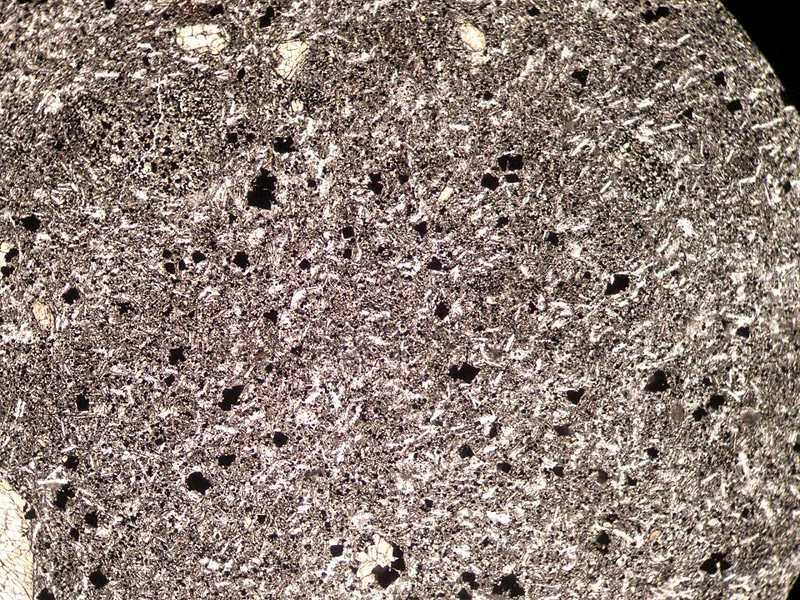
\includegraphics[height=3.6cm]{images/book2/g11-chmee2-basalt-ppl.jpg}\hfill
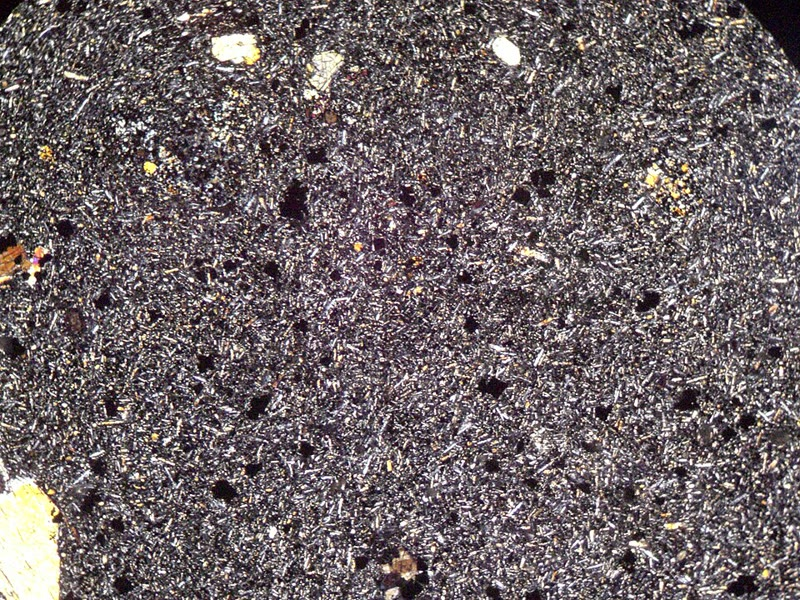
\includegraphics[height=3.6cm]{images/book2/g11-chmee2-basalt-xpl.jpg}\hfill
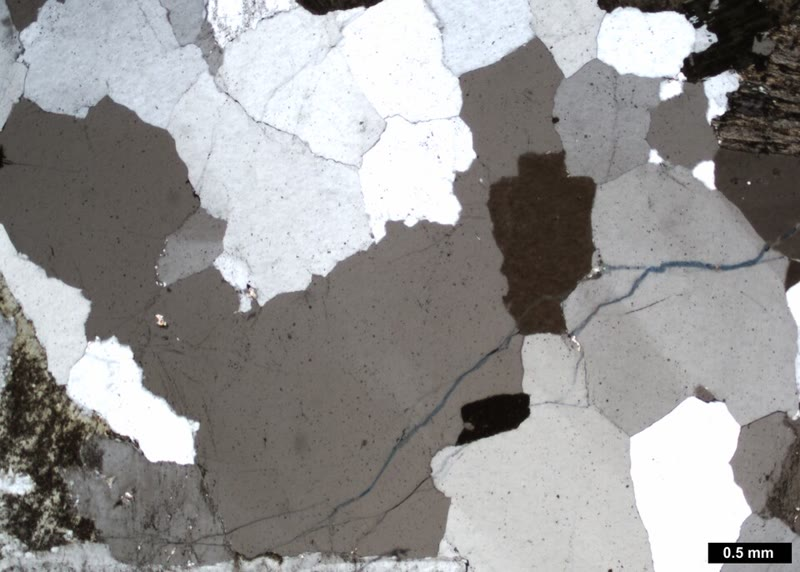
\includegraphics[height=3.6cm]{images/book2/g11-rygel-granite-xpl.jpg}

{\small À gauche et au centre~: le même basalte en \omterm{def:g11:minerals:thin-section}{lame mince}, en lumière
polarisée non analysée et entre polariseurs croisés. La roche est à grain
fin~: de petits cristaux allongés, surtout de plagioclase, et des taches
noires qui ne laissent passer aucune lumière dans les deux cas~; entre
polariseurs croisés, les cristaux s'illuminent en gris et en couleurs.
Photographies
Chmee2 (CC~BY-SA~3.0). À droite~: des cristaux de quartz dans un granite,
entre polariseurs croisés, chacun dans sa propre nuance de gris (la barre
d'échelle mesure \qty{0.5}{mm}). Photographie Michael C.~Rygel
(CC~BY-SA~3.0).}
\end{omfigure}
% ledger: photo:g11-basalt-thin-section, photo:g11-granite-thin-section

En lumière polarisée non analysée, une \omterm{def:g11:minerals:thin-section}{lame mince} ressemble à un vitrail~:
la plupart des minéraux sont presque incolores, certains teintés, et les
contours des grains, leurs \omterm{def:g11:minerals:cleavage}{clivages} et leurs \omterm{def:g11:minerals:habit}{habitus} apparaissent
nettement. Entre polariseurs croisés, les filtres, orientés en travers l'un
de l'autre, ne laisseraient à eux seuls passer aucune lumière~; la plupart
des minéraux modifient la lumière qui les traverse, et apparaissent en
nuances de gris ou en couleurs vives, qui changent quand on tourne la lame.
Deux grains d'un même minéral peuvent avoir un aspect différent, parce que
chacun est coupé selon sa propre direction~: les grains de quartz du granite
ci-dessus sont tous du quartz, en nuances différentes. Les couleurs, leurs
changements et ce qu'elles révèlent de chaque minéral sont l'objet de la
première année d'université~; ici, la \omterm{def:g11:minerals:thin-section}{lame mince} est une image de la roche,
dans laquelle chaque grain peut être vu, nommé et compté.

\section{Exercices}

\begin{exercise}[$\star$]\label{exo:g11:minerals:1}
Définir le \omterm{def:g11:minerals:cleavage}{clivage} et la \omterm{def:g11:minerals:cleavage}{cassure}. Lequel des deux le quartz montre-t-il, et
à quoi ressemblent ses surfaces de rupture~? Combien de \omterm{def:g11:minerals:cleavage}{clivages} un mica
possède-t-il~?
\end{exercise}

\begin{exercise}[$\star$]\label{exo:g11:minerals:2}
Pourquoi la couleur est-elle un mauvais guide pour identifier le quartz,
mais un assez bon guide pour l'olivine~? Donner deux propriétés plus fiables
que la couleur.
\end{exercise}

\begin{exercise}[$\star$]\label{exo:g11:minerals:3}
Associer chaque description à un minéral parmi le quartz, l'orthose, la
biotite et l'olivine~: (1) des grains verts dans un basalte~; (2) des
paillettes noires qui se détachent en feuillets minces~; (3) des grains
roses et trapus à deux plans de rupture plans, rayés par un clou
d'acier~; (4) des grains gris et vitreux à \omterm{def:g11:minerals:cleavage}{cassures} courbes, non rayés par
le clou.
\end{exercise}

\begin{exercise}[$\star$]\label{exo:g11:minerals:4}
(1) Combien d'atomes un \omterm{def:g11:minerals:silicate}{tétraèdre silicium--oxygène} contient-il, et où
sont-ils~? (2) À l'aide des charges des ions \ce{Si^4+} et \ce{O^2-},
trouver la charge du groupe \ce{SiO4}.
\end{exercise}

\begin{exercise}[$\star$]\label{exo:g11:minerals:5}
Nommer les six groupes de \omterm{def:g11:minerals:rock-forming}{silicates constitutifs des roches} et donner, pour
chacun, la façon dont ses tétraèdres sont reliés.
\end{exercise}

\begin{exercise}[$\star\star$]\label{exo:g11:minerals:6}
Les masses atomiques du silicium et de l'oxygène valent \qty{28.085}{g/mol}
et \qty{15.999}{g/mol}. (1) Calculer la part de l'oxygène dans la masse du
quartz, \ce{SiO2}. (2) Faire de même pour la forstérite, l'olivine
magnésienne \ce{Mg2SiO4} (magnésium~: \qty{24.305}{g/mol}). (3) Comparer à
la part de l'oxygène dans la croûte continentale, environ
\qty{46}{\percent}.
\end{exercise}

\begin{exercise}[$\star\star$]\label{exo:g11:minerals:7}
Un grain blanc d'un granite raye une plaque de verre (environ 5.5) mais il
est rayé par un clou d'acier (environ 6.5)~; il se casse selon des plans
dans deux directions. Un second grain, gris, n'est pas rayé par le clou et
se casse selon des surfaces courbes. Identifier les deux, en donnant les
raisons.
\end{exercise}

\begin{exercise}[$\star\star$]\label{exo:g11:minerals:8}
Dans le pyroxène augite, chaque tétraèdre partage deux sommets. (1) À
l'aide de la proposition sur le comptage des oxygènes, combien y a-t-il
d'oxygènes pour chaque silicium~? (2) Vérifier que la partie
\ce{(Si,Al)2O6} de la formule de l'augite concorde.
\end{exercise}

\begin{exercise}[$\star\star$]\label{exo:g11:minerals:9}
Un basalte est fait, en volume, de \qty{55}{\percent} de labradorite
(\qty{2.69}{g/cm^3}), de \qty{35}{\percent} d'augite (\qty{3.4}{g/cm^3}) et
de \qty{10}{\percent} d'olivine (\qty{3.32}{g/cm^3}). Calculer sa masse
volumique, puis la masse d'un cube de ce basalte de \qty{10}{cm} de côté.
\end{exercise}

\begin{exercise}[$\star\star$]\label{exo:g11:minerals:10}
Une \omterm{def:g11:ocean-ridges:peridotite}{péridotite} du manteau est faite de \qty{75}{\percent} d'olivine
(\qty{3.32}{g/cm^3}) et de \qty{25}{\percent} d'augite (\qty{3.4}{g/cm^3}).
(1) Calculer sa masse volumique. (2) De quel pourcentage est-elle plus
dense que le basalte de l'exercice précédent, à environ \qty{3.00}{g/cm^3}~?
(3) Pourquoi la \omterm{def:g11:ocean-ridges:oceanic-lithosphere}{croûte océanique} reste-t-elle au-dessus du manteau~?
\end{exercise}

\begin{exercise}[$\star\star$]\label{exo:g11:minerals:11}
Sur une \omterm{def:g11:minerals:thin-section}{lame mince} d'une roche, une grille de 400 points tombe 168 fois sur
du plagioclase, 132 fois sur du pyroxène, 60 fois sur de l'olivine et
40 fois sur des trous laissés par des bulles de gaz. (1) Calculer la
fraction de chacun. (2) Pourquoi ne peut-on pas appliquer directement la
proposition sur la masse volumique d'une roche à toute la lame~?
(3) Calculer la masse volumique de la partie solide, avec \qty{2.69}{},
\qty{3.4}{} et \qty{3.32}{g/cm^3}, puis celle de la roche avec ses trous.
\end{exercise}

\begin{exercise}[$\star\star\star$]\label{exo:g11:minerals:12}
Dans \qty{1}{kg} de croûte continentale, il y a environ \qty{464}{g}
d'oxygène, \qty{283}{g} de silicium, \qty{84}{g} d'aluminium, \qty{52}{g}
de fer, \qty{46}{g} de calcium, \qty{28}{g} de magnésium, \qty{23}{g} de
sodium et \qty{15}{g} de potassium. Les masses atomiques valent
\qty{16.0}{}, \qty{28.1}{}, \qty{27.0}{}, \qty{55.8}{}, \qty{40.1}{},
\qty{24.3}{}, \qty{23.0}{} et \qty{39.1}{g/mol}. (1) Calculer le nombre de
moles de chaque élément. (2) Quelle fraction des atomes de la croûte sont
des atomes d'oxygène~? (3) Pourquoi décrit-on parfois la croûte comme un
empilement d'ions oxygène, les autres éléments occupant les espaces qui les
séparent~?
\end{exercise}

\begin{exercise}[$\star\star\star$]\label{exo:g11:minerals:13}
Dans une chaîne double d'amphibole, la moitié des tétraèdres partagent deux
sommets et l'autre moitié trois. (1) Combien y a-t-il d'oxygènes pour chaque
silicium~? (2) Écrire le résultat pour quatre siliciums. (3) Dans la
formule de la hornblende,
\ce{Ca2[Mg4(Al,Fe)]Si7AlO22(OH)2}, l'aluminium prend la place du silicium
dans un tétraèdre sur huit. Vérifier que la formule concorde.
\end{exercise}

\begin{exercise}[$\star\star\star$]\label{exo:g11:minerals:14}
Dans la Sierra Nevada de Californie, \num{6454} échantillons de roches
granitiques ont une masse volumique moyenne de \qty{2.69}{g/cm^3}~; elle
dépasse \qty{2.7}{g/cm^3} à l'ouest, et descend sous \qty{2.6}{g/cm^3} là où
le granite est le plus riche en silice et en potassium. Calculer la masse
volumique d'une roche à \qty{20}{\percent} de quartz
(\qty{2.62}{g/cm^3}), \qty{10}{\percent} d'orthose (\qty{2.56}{}),
\qty{50}{\percent} d'oligoclase (\qty{2.65}{}), \qty{10}{\percent} de
biotite (\qty{3.09}{}) et \qty{10}{\percent} de hornblende (\qty{3.23}{}).
Comparer au granite de l'exemple de ce chapitre, et expliquer le contraste
entre les deux parties de la Sierra Nevada.
\end{exercise}

\begin{exercise}[$\star\star\star$]\label{exo:g11:minerals:15}
La croûte continentale supérieure contient environ \qty{66.6}{\percent} de
\ce{SiO2} en masse, la croûte continentale dans son ensemble
\qty{60.6}{\percent}. (1) À l'aide de la part du silicium dans \ce{SiO2}
(\qty{46.7}{\percent}), calculer dans chaque cas la part de silicium
contenue dans \ce{SiO2}. (2) Quels minéraux s'attendrait-on à trouver plus
souvent dans la croûte supérieure que plus bas~? (3) Qu'est-ce que cela
implique pour la masse volumique de la croûte supérieure par rapport à la
croûte plus profonde~?
\end{exercise}

\section{Problème~: la masse volumique d'un granite}

\begin{problem}[{Problème du week-end --- d'un comptage de points à une masse volumique}]
\label{pb:g11:minerals:1}
% values (mineral_density.py): GRANITE_COUNT 150/175/125/30/20; rho_granite 2.6427;
% granite_air_g 264.27, granite_water_g 164.27; densities wm:densities; usgs91:sierra
Un bloc de granite rose est scié et poli. On identifie ses minéraux, on les
compte sur une grille, et l'on calcule la masse volumique de la roche, que
l'on vérifie ensuite par pesée.

\medskip
\noindent\textbf{Partie I --- Identifier les minéraux.}
\begin{enumerate}
  \item Les grains A sont gris et vitreux, ne montrent aucune surface de
        rupture plane, seulement des surfaces courbes, et ne sont pas rayés
        par un clou d'acier. De quel minéral s'agit-il~?
  \item Les grains B sont roses et trapus, se cassent selon des plans
        brillants dans deux directions, rayent le verre mais sont rayés par
        le clou. De quel minéral s'agit-il, et quelle est sa dureté sur
        l'échelle de Mohs~?
  \item Les grains C ont la même dureté et les mêmes \omterm{def:g11:minerals:cleavage}{clivages} que les
        grains B, mais ils sont blancs~; une analyse y trouve du sodium et
        du calcium, et pas de potassium. De quelle sorte de feldspath
        s'agit-il~?
  \item Les grains D sont des paillettes noires, les grains E des
        paillettes argentées~; tous deux se détachent en feuillets minces.
        De quels minéraux s'agit-il, et quel trait de leur structure
        explique les feuillets~?
  \item Lesquels des minéraux A à E sont des \omterm{def:g11:minerals:silicate}{silicates} en charpente~?
        Lesquels contiennent du fer et du magnésium~?
\end{enumerate}

\medskip
\noindent\textbf{Partie II --- Le comptage de points.}
\begin{enumerate}[resume]
  \item Une grille de 500 points tombe 150 fois sur du quartz, 175 fois sur
        de l'orthose, 125 fois sur de l'oligoclase, 30 fois sur de la
        biotite et 20 fois sur de la muscovite. Calculer la fraction de
        chaque minéral.
  \item Pourquoi la fraction des points estime-t-elle la fraction du volume
        de la roche~?
  \item Quel pourcentage de la roche est du feldspath~?
  \item Si un point est mal compté, de combien une fraction change-t-elle~?
  \item Cette roche est-elle un granite au sens du livre~1~?
\end{enumerate}

\medskip
\noindent\textbf{Partie III --- La masse volumique.}
\begin{enumerate}[resume]
  \item Énoncer la formule qui donne la masse volumique d'une roche sans
        pores à partir de ses minéraux.
  \item Avec les masses volumiques quartz \qty{2.62}{}, orthose
        \qty{2.56}{}, oligoclase \qty{2.65}{}, biotite \qty{3.09}{} et
        muscovite \qty{2.82}{g/cm^3}, calculer la contribution
        $\phi_i \rho_i$ de chaque minéral.
  \item Les additionner~: quelle est la masse volumique du granite~?
  \item Quel minéral contribue le plus à la somme~? Quels sont les deux
        minéraux qui, bien qu'ils ne forment qu'un dixième de la roche,
        augmentent sa masse volumique~?
  \item Convertir la masse volumique en \unit{kg/m^3}, et donner la masse
        d'\qty{1}{m^3} de ce granite.
\end{enumerate}

\medskip
\noindent\textbf{Partie IV --- La vérification par pesée.}
\begin{enumerate}[resume]
  \item On scie dans le granite un bloc de \qty{100}{cm^3}. Quelle masse
        s'attend-on à lui trouver~?
  \item Suspendu dans l'eau, un corps est poussé vers le haut par le poids
        de l'eau qu'il déplace (les livres de physique). Quelle masse la
        balance indique-t-elle quand le bloc est suspendu entièrement
        immergé dans l'eau, de masse volumique \qty{1.00}{g/cm^3}~?
  \item Les laboratoires calculent la masse volumique d'un échantillon de
        roche par
        $m_{\text{air}}/(m_{\text{air}} - m_{\text{eau}})$. Vérifier que
        vos deux masses redonnent la masse volumique de la question~13.
  \item Les roches granitiques de la Sierra Nevada ont en moyenne une masse
        volumique de \qty{2.69}{g/cm^3}, et celles qui sont les plus riches
        en silice et en potassium sont en dessous de \qty{2.6}{g/cm^3}. Où
        se situe ce granite, et quels minéraux rendraient un granite plus
        dense~?
  \item Conclure~: quelle est la masse volumique du granite~?
\end{enumerate}
\end{problem}
